\chapter{Evaluation}
\label{chapter:evaluation}

The accuracy evaluation of each step is described in this chapter.

% \begin{figure}[h]
%     \centering
%     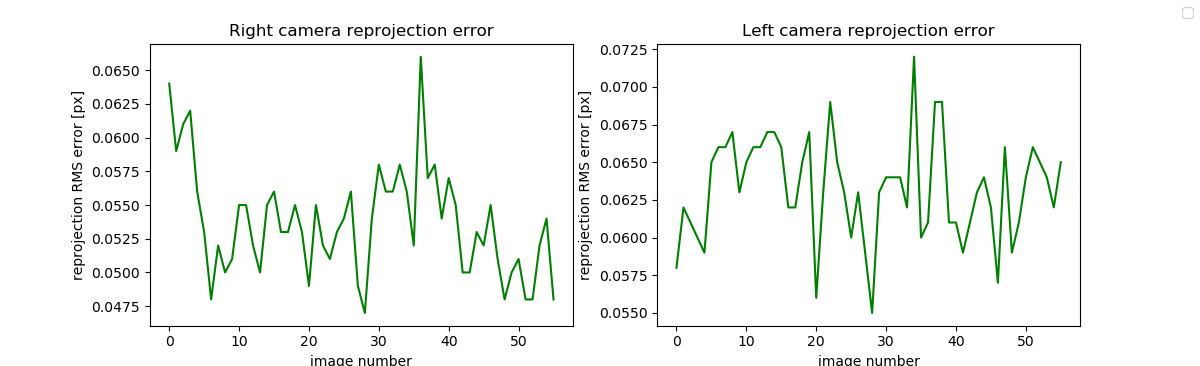
\includegraphics[width=\textwidth]{graphics/single_cam_calib.png}
%     \caption{The output of the ROS calibration checking tool.}
%     \label{fig:camcheck}
% \end{figure}

For computing the error of each camera calibration, another tool from the same ROS Camera Calibration package is used.
It outputs a reprojection $\mathsf{RMS}$ error, which stands for Root-mean-square error and can be defined As
\begin{equation}
    \mathsf{RMS}(x | \hat{x} ) = \sqrt{\frac{\sum_{i=1}^{N}{(x_i - \hat{x}_i)^2}}{N}}
\end{equation}

Where $x$ is a measured data sample from the experiment, $\hat{x}$ is a ground-truth data and $N$ is a sample size.
The reprojection error varies depending on the pose of the chessboard with an upper bound of less than $1$px.
